\def\logooffset{271}
\def\phylogo{
\includegraphics[height=15.605mm]{ph-logo.pdf}}
\def\E18Logo{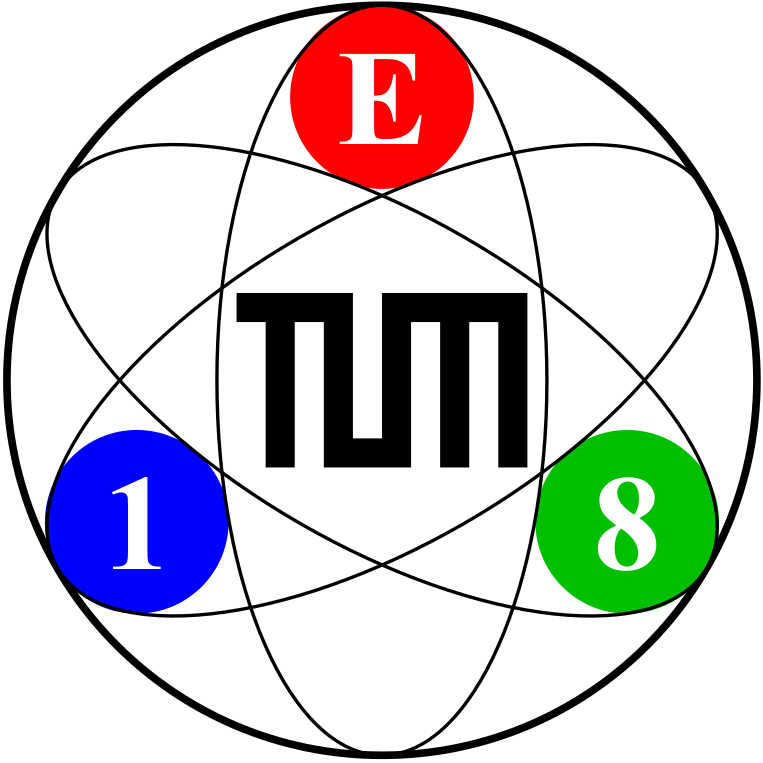
\includegraphics[height=15.605mm]{E18Logo.png}}
\def\tumlogo{
\includegraphics[height=15.605mm]{Tum_logo.png}} % optional MSE logo
\def\deadline{January 2025} 					% month and year of submission
\def\title{Development of FPGA based frontend electronics for the scintillating fiber hodoscope of the AMBER experiment at CERN}   				% title of the thesis
\def\author{Tim Maehrholz}							% your name
\def\typeOfThesis{Bachelor's Thesis}   		

\renewcommand\maketitle{
\begin{titlepage}
	\vspace*{1.0cm}%
	\noindent
	\begin{picture}(0,0)(25,\logooffset)
    	\put(25,272){\phylogo}					% 25,272
    	\put(90,272){\E18Logo}
    	\put(410,272){\tumlogo}					% 176,272
	\end{picture}%
  
	\vspace*{1.5cm}%

	\noindent\fontsize{12}{16}\selectfont\rmfamily Institute for Hadronic Structure and Fundamental Symmetries\\
	School of Natural Sciences\\
	Technical University of Munich
	
	\vspace*{2cm} 
	% Anpassung der Schriftgroesse des Titels exakt 15 - Durchschuss 20
	\begin{center}
		{\color{tumblauTitel}
		\noindent\fontsize{20.74}{26}\selectfont\rmfamily\textbf{\title}
		}

		\vspace{2cm}
		% author
		\noindent\fontsize{17.28}{22}\selectfont\textbf{\author}
  
		\vspace{0.5cm}
		\noindent\fontsize{12}{16}\selectfont\rmfamily\typeOfThesis
		%\vspace{20\baselineskip}

		\vspace{2cm}
		Supervisor: \\
		\noindent\fontsize{12}{16}\selectfont\rmfamily\textbf{Prof. Dr.} \\
		Chair of 

		\vspace{0.5cm}

		Second Examiner: \\
		\noindent\fontsize{12}{16}\selectfont\rmfamily{PD Dr. } \\



    	\vfill
    	\noindent\deadline
	\end{center}
\end{titlepage}
}